\documentclass[aspectratio=169]{beamer}
\usetheme{metropolis}
\usecolortheme[snowy]{owl}

%Information to be included in the title page:
\title{Astrape --- Anonymous Payment Channels With Boring Cryptography}
\author{Yuhao Dong}
\institute{University of Waterloo}
\date{\today}
 

\begin{document}

\frame{\titlepage}

\section{Introduction}

\begin{frame}{The problem with blockchains}
    Blockchain-based cryptocurrencies promise to revolutionarize money.
    \begin{itemize}
        \item Decentralized
        \item Censorship-resistant
        \item Completely permissionless
    \end{itemize}

    Unfortunately, blockchains aren't a very good money ledger:
    \begin{itemize}
        \item Lack of privacy --- can render censorship resistance meaningless
        \item Very poor transaction throughput
    \end{itemize}
\end{frame}

\begin{frame}{The problem with blockchains}
    One way of fixing this is by improving blockchains
    \begin{itemize}
        \item Privacy: Zcash, Monero, etc
              \begin{itemize}
                  \item Terrible performance!
              \end{itemize}
        \item Scalability: sharding, dPoS, etc
              \begin{itemize}
                  \item Complexity/centralization
              \end{itemize}
    \end{itemize}

    A better way: \textbf{payment channels}
\end{frame}

\begin{frame}{Payment channels}
    What is a payment channel?
    \begin{itemize}
        \item Alice and Bob each lock \$50 into a vault.
        \item When transactions happen between Alice and Bob, they privately sign a statement saying which of the \$100 belongs to Alice, and which to Bob.
        \item Vault can be opened by a signed statement from both Alice and Bob declaring the correct split. But this statement can be overridden with newer statements within a timeout period.
    \end{itemize}

    \textbf{Payment channel networks} are mesh networks of users with payment channels open to their neighbors. Transactions are passed through multiple intermediaries.
    \begin{itemize}
        \item Horizontal scalability!
    \end{itemize}
\end{frame}

\begin{frame}{Atomic multi-hop transactions}
    Payment channel networks require an \textbf{atomic multi-hop transaction} construction.
    \begin{itemize}
        \item Pay Alice so that she pays Bob so that he pays Carol
        \item Ensure that money cannot be stolen by intermediaries
    \end{itemize}

    Most common construction: \textbf{hash time-lock contract} (HTLC).
    \begin{itemize}
        \item \$100 payable to:
              \begin{itemize}
                  \item Bob if he can find $p$ such that $H(p) = x$ within $t$ hours
                  \item Alice otherwise
              \end{itemize}
    \end{itemize}

    Thus, Alice can randomly generate $p,x$ tell Carol the answer to the puzzle, then send Bob an HTLC. Bob will send Carol an analogous HTLC. Carol solves the puzzle to claim the money, letting Bob claim the money from Alice.
\end{frame}

\begin{frame}{Problems with HTLC}
    The biggest problem with HTLC is \textbf{poor privacy}
    \begin{itemize}
        \item All intermediaries receive coins with the same puzzle.
        \item Different hops know they're on the same transaction.
        \item Can lead to deanonymization!
    \end{itemize}

    Existing work on fixing HTLC does exist:
    \begin{itemize}
        \item Specialized protocols for special blockchains (Bolt for ZCash, etc)
        \item Fulgor (Malavolta et al. 2017) --- expensive, off-chain zero-knowledge proofs, but compatible with most blockchains
        \item Tumblebit (Goldberg et al. 2017) --- custom construction based on RSA
        \item AMHL (Malavolta et al. 2019) --- on-chain linear homomorphic encryption
    \end{itemize}
\end{frame}

\begin{frame}{Why not existing solutions?}
    No anonymous PCN construction exists with only HTLC's cryptography
    \begin{itemize}
        \item \textbf{Black-box} signature \& hash
    \end{itemize}

    All are tightly coupled to the mathematics of specific constructions
    \begin{itemize}
        \item You can't ``swap out'' RSA with e.g. SPHINCS in Tumblebit
    \end{itemize}
\end{frame}


\section{Astrape: our construction}

\begin{frame}{Astrape}
    Astrape is a novel anonymous PCN construction that uses the same tools as HTLC --- generic hash functions and signatures.

    Three objectives:
    \begin{itemize}
        \item \textbf{Relationship anonymity}: Given two simultaneous payments of the same value with paths sharing an honest intermediary, an attacker cannot know which individual transactions belong to which payment pay even if all other intermediaries are compromised.
        \item \textbf{Balance security}: No honest user ever loses money involuntarily.
        \item \textbf{Wormhole resistance}: Attackers cannot make a payment ``skip'' intended intermediaries to deprive them of fees.
    \end{itemize}

    ``Onion-routing-like'' anonymity, similar to Tumblebit and AMHL
\end{frame}

\begin{frame}{Notation and framework}
    We ignore other aspects of a PCN and focus on atomic multi-hop transactions.
    \begin{itemize}
        \item $U_0$ wishes to pay $U_n$ through intermediaries $U_1,\dots,U_{i-1}$.
        \item We denote the \textbf{coin} that $U_i$ sends to $U_{i+1}$ as $U_i \rightarrow U_{i+1}$
        \item Each coin has a \textbf{lock} --- a boolean function representing a puzzle that the recipient must solve. For example, we might represent an HTLC as:
              \begin{multline*}
                  \mathsf{HTLC}[x,t,A,B] \; ::= \; (\pi,\zeta) \mapsto \\
                  (H(\pi)=x \land \mathsf{Signed}_B(\zeta)) \lor
                  (\mathsf{Timeout}[t]\land\mathsf{Signed}_A(\sigma))
              \end{multline*}
    \end{itemize}
\end{frame}

\begin{frame}{Multi-hop HTLC}
    We first construct a ``strawman'' construction that doesn't work --- multi-hop HTLC.

    \begin{itemize}
        \item The sender $U_0$ samples random values $(r_1,\dots,r_n)$ and calculates $s_i=H(r_i\oplus r_{i+1}\oplus\dots\oplus r_n)$.
        \item $U_0$ then sends $(r_i,s_i,[s_{i+1}])$ to $U_i$
        \item Each coin $U_{i} \rightarrow U_{i+1}$ is locked by $\mathsf{HTLC}[s_{i+1},t,U_i,U_{i+1}]$
    \end{itemize}

    The recipient $U_{n}$ can solve the HTLC on $s_n$. This enables $U_{n-1}$ to solve its puzzle and so on and so forth:
    \[ H^{-1}(s_i) = r_i \oplus H^{-1}(s_{i+1}) \]
\end{frame}

\begin{frame}{Multi-hop HTLC}
    Multi-hop HTLC does have \textbf{relationship anonymity}
    \begin{itemize}
        \item Intuitively, because given a random-oracle hash function, $s_i$ and $s_j$ are random-looking and cannot be correlated
    \end{itemize}

    Unfortunately, it has no \textbf{balance security}!
    \begin{itemize}
        \item Malicious $U_0$ can give some intermediary $U_i$ a false $r_i$.
        \item When $U_i \rightarrow U_{i+1}$ is spent, $U_i$ finds that he cannot spend $U_{i-1} \rightarrow U_i$.
        \item $U_n$ will get paid with $U_i$'s money instead of $U_0$'s!
    \end{itemize}

    ``Bad state'' attack

    Fulgor (Malavolta et al. 2017) is simply multi-hop HTLC plus a zero-knowledge proof that $U_0$ gives each hop that $U_0$ isn't lying. We can do better.
\end{frame}

\begin{frame}{Fixing multi-hop HTLC}
    Our central insight: \emph{corrupt senders need no privacy}.
    \begin{itemize}
        \item If the attacker corrupts the sender he already broke all privacy guarantees
        \item Sender \emph{already knows the whole path} in our model
    \end{itemize}

    Thus, we can compose multi-hop HTLC with a \textbf{non-anonymous} mechanism
    \begin{itemize}
        \item that's only triggered when the sender is corrupt
        \item and doesn't leak information unless used
    \end{itemize}

    This isn't particularly hard to do with ``boring'' crypto.
\end{frame}

\begin{frame}{Constructing fraud proofs}
    After generating the multi-hop HTLC parameters, $U_0$ generates $n$ values $x_i$ recursively:
    \begin{align*}
        x_i & = H(r_i||s_i||s_{i+1}||o_i||x_{i+1}) \\
        x_n & = H(o_n)
    \end{align*}
    where $o_i$ is a random nonce.

    The intuition here is that $x_i$ commits to all the information the sender would give to all hops $U_j$ where $j\geq i$.

    $x_i$ is then given to $U_i$.
\end{frame}

\begin{frame}{Constructing fraud proofs}
    Let's consider what happens if $U_0$ attempts to defraud $U_i$ by giving it the wrong $r_i$. This generates the following \textbf{fraud proof} $\{k_{i+1}, r_i, s_i, s_{i+1}, o_i \}$ where:
    \begin{gather*}
        H(k_{i+1}) = s_i \\
        H(r_i\oplus(k_{i+1}) \neq s_i\\
        H(r_i||s_i||s_{i+1}||o_i||x_{i+1})=x_i
    \end{gather*}

    that can be verified by anybody with $x_i$, like $U_i$.

    $(k_{i+1}$ would be the HTLC solution $H^{-1}(s_i)$ that $U_i \rightarrow U_{i+1}$ was spent with.
\end{frame}

\begin{frame}{Constructing fraud proofs}
    Since $x_i$ commits to \emph{all} multi-hop HTLC initialization states ``rightwards'' of $U_i$, $U_i$, in cooperation with $U_{i-1}$, can also produce a fraud proof that $U_{i-2}$ can verify using $x_{i-2}$. This is a set of simply $\lambda$-bit values $k_{i+1}$, $r_{i-1}$, $s_{i-1}$, $r_i$, $s_i$,$s_{i+1}$, $x_i$, $x_{i+1}$ where:
    \begin{align*}
        H(k_{i+1})                               & = s_{i+1} \\
        H(r_i \oplus k_{i+1})                    & \neq s_i  \\
        H(r_i||s_i||s_{i+1}||o_i||x_{i+1})       & = x_i     \\
        H(r_{i-1}||s_{i-1}||s_{i}||o_{i-1}||x_i) & = x_{i-1}
    \end{align*}

    We can extend this idea all the way back to $U_0$.
\end{frame}

\begin{frame}{Constructing Astrape: Initialization}
    We are now ready to present an informal definition of Astrape's protocol

    First, $U_0$ derives:
    \begin{itemize}
        \item Random strings $(r_1,\dots,r_n)$ and $(o_1,\dots,o_n)$
        \item $s_i=H(r_i\oplus r_{i_1}\oplus\dots \oplus r_n)$
        \item $x_i=H(r_i||s_i||s_{i+1}||o_i||x_{i+1}); x_n=H(o_n)$
    \end{itemize}

    $U_0$ then sends to each hop $U_i$ the tuple $(r_i,s_i,s_{i+1},x_i,x_{i+1},o_i)$

    The last hop $U_n$ gets $(r_n,s_n,x_n,o_n)$.
\end{frame}

\begin{frame}{Constructing Astrape: Sending the coins}
    Each $U_i$ then sends to its successor $U_{i+1}$ the coin $U_i \rightarrow U_{i+1}$.

    This is locked with a script that allows the coin to be spent by one of two ways:
    \begin{itemize}
        \item Solving a multi-hop HTLC on $r_i$ (the ``normal'' case)
        \item Presenting a fraud proof for any ``downstream'' hop, with enough information to convince anyone possessing $x_i$. (the ``fraud'' case)
    \end{itemize}

\end{frame}

\begin{frame}{Constructing Astrape: Spending the coins}
    After receiving a coin from $U_{n-1}$, $U_n$ spends it by solving the multi-hop HTLC clause with $\pi=r_n$.

    Each intermediate node $U_i$ reacts when its right coin $U_i \rightarrow U_{i+1}$ gets spent:
    \begin{itemize}
        \item If $U_{i+1}$ spent the HTLC case with $(k_{i+1})$, construct $k_i = r_i \oplus k_{i+1}$
              \begin{itemize}
                  \item If $\pi'$ can spend the HTLC case for our incoming $U_{i-1} \rightarrow U_i$ coin, broadcast a transaction spending it.
                  \item Otherwise, $U_i$ must have lied to us! Construct fraud proof and spend the fraud case of our incoming coin.
              \end{itemize}
        \item Otherwise, $U_{i+1}$ spent the fraud case with a valid fraud proof somewhere down the line.
              \begin{itemize}
                  \item We solve the fraud case of our incoming coin by copying all the parameters, except adding on all our parameters so that it can be verified by our predecessor.
              \end{itemize}
    \end{itemize}

    This continues until all coins are spent.
\end{frame}


\section{Discussion and evaluation}

\begin{frame}{Does Astrape accomplish our goals?}
    Astrape accomplishes all three goals:
    \begin{itemize}
        \item \textbf{Relationship anonymity}: harder to prove than with Fulgor/multi-hop HTLC, due to the complexity in the Collapse case. Hinges on inability to correlate $x_i$ and $x_j$ as long as $j > x + 1$.
        \item \textbf{Balance security}: $U_i \rightarrow U_{i+1}$ being spent always leads to $U_{i-1} \rightarrow U_i$ being spendable.
        \item \textbf{Wormhole resistance}: yes, because $U_{i-1} \rightarrow U_i$ can only be spent if $U_i \rightarrow U_{i+1}$ is spent, assuming $U_{i+1}$ and the sender are honest.
    \end{itemize}
\end{frame}

\begin{frame}{Performance}
    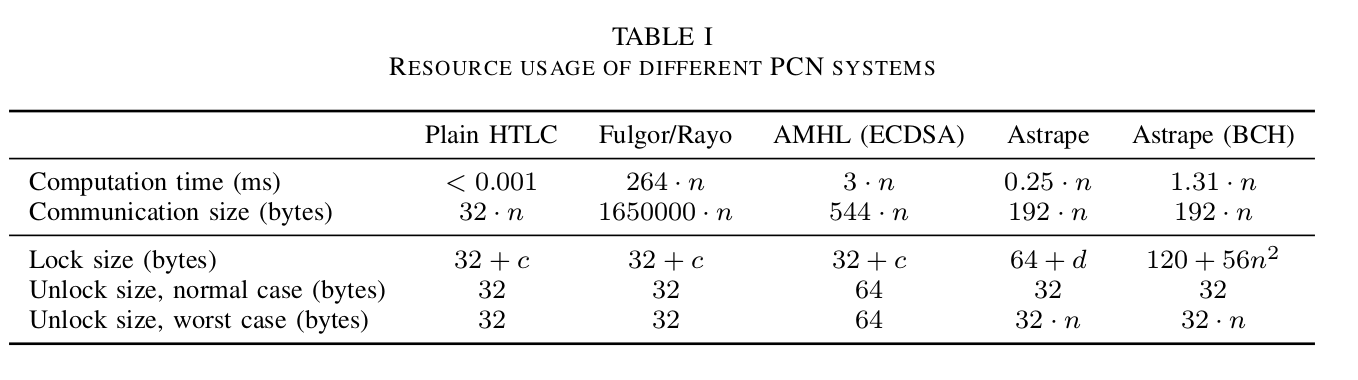
\includegraphics[width=\textwidth]{table.png}
\end{frame}

\section{Conclusion}

\begin{frame}
    Astrape achieves strong anonymity and high performance while using only black-box access to a secure hash function and signature scheme.

    This solves a significant open problem in the field --- ``what are the basic cryptographic building blocks needed for anonymous multi-hop transactions'' (Malavolta 2019)
    \begin{itemize}
        \item Answer: the same building blocks needed for ``usual'' multi-hop transactions
    \end{itemize}

    We can easily deploy Astrape on legacy blockchains like Bitcoin Cash at high performance.
\end{frame}

\section{Questions?}

\end{document}

